\documentclass[a4paper,11pt]{article}
\usepackage{latexsym}
\usepackage{xcolor}
\usepackage{float}
\usepackage{ragged2e}
\usepackage[empty]{fullpage}
\usepackage{wrapfig}
\usepackage{lipsum}
\usepackage{tabularx}
\usepackage{titlesec}
\usepackage{geometry}
\usepackage{marvosym}
\usepackage{verbatim}
\usepackage{enumitem}
\usepackage[hidelinks]{hyperref}
\usepackage{fancyhdr}
\usepackage{fontawesome5}
\usepackage{multicol}
\usepackage{graphicx}
\usepackage{cfr-lm}
\usepackage[T1]{fontenc}
\usepackage{tikz}
\usepackage{titling}
\setlength{\multicolsep}{0pt} 
\pagestyle{fancy}
\fancyhf{} % clear all header and footer fields
\fancyfoot{}
\renewcommand{\headrulewidth}{0pt}
\renewcommand{\footrulewidth}{0pt}
\geometry{left=1.4cm, top=0.8cm, right=1.2cm, bottom=1cm}

\usepackage[most]{tcolorbox}
\tcbset{
	frame code={},
	center title,
	left=0pt,
	right=0pt,
	top=0pt,
	bottom=0pt,
	colback=gray!20,
	colframe=white,
	width=\dimexpr\textwidth\relax,
	enlarge left by=-2mm,
	boxsep=4pt,
	arc=0pt,outer arc=0pt,
}

\urlstyle{same}
\raggedright
\setlength{\tabcolsep}{0in}

% Sections formatting
\titleformat{\section}{
  \vspace{-4pt}\scshape\raggedright\large
}{}{0em}{}[\color{black}\titlerule \vspace{-6pt}]

%-------------------------
% Custom commands

\newcommand{\resumeItem}[2]{
  \item{
    \textbf{#1}{\hspace{0.5mm}#2 \vspace{-0.5mm}}
  }
}

% 5-argument Experience block: Company, Location, Role, Dates, Tech
\newcommand{\resumeExperience}[5]{
  \vspace{1mm}\item
    \begin{tabular*}{0.98\textwidth}[t]{l@{\extracolsep{\fill}}r}
        \textbf{#1} & \textit{\footnotesize{#4}} \\
        {\footnotesize{#3}} & \footnotesize{#2}
    \end{tabular*}
    \vspace{1mm}
    \parbox{0.98\textwidth}{\footnotesize #5}
    \vspace{-4.2mm}
}

% 3-argument Project block: Title, Dates, Tech/Details
\newcommand{\resumeProject}[3]{
  \vspace{1mm}\item
  \begin{tabular*}{0.98\textwidth}[t]{l@{\extracolsep{\fill}}r}
    \textbf{#1} & \textit{\footnotesize{#2}} \\
    \multicolumn{2}{l}{\footnotesize{#3}}
  \end{tabular*}
  \vspace{-3.4mm}
}

% 5-argument Education block: Degree, Detail, Additional, Program/Focus, Dates
\newcommand{\resumeEducation}[5]{
  \vspace{1mm}\item
    \begin{tabular*}{0.98\textwidth}[t]{l@{\extracolsep{\fill}}r}
        \textbf{#1}{\footnotesize #2} & \textit{\footnotesize{#5}} \\
        {\footnotesize{#4}} &  \footnotesize{#3}\\
    \end{tabular*}
    \vspace{0.5mm}
}

\newcommand{\resumeSubItem}[2]{
  \vspace{2.4mm}
    \begin{tabular*}{0.98\textwidth}[t]{l@{\extracolsep{\fill}}r}
        \footnotesize{\textit{#1}} & \footnotesize{\textit{#2}}
    \end{tabular*}
    \vspace{-0.8mm}
}

\newcommand{\resumeProjectSubheader}[2]{
  \item[] {\hspace*{-3ex}\textbf{#1} | \textit{#2}}
}

\renewcommand{\labelitemi}{$\vcenter{\hbox{\tiny$\bullet$}}$}

\newcommand{\resumeSubHeadingListStart}{\begin{itemize}[leftmargin=*,label={},labelsep=0mm]}
\newcommand{\resumeHeadingSkillStart}{\begin{itemize}[leftmargin=*,itemsep=1.7mm, rightmargin=2ex]}
\newcommand{\resumeItemListStart}{\begin{justify}\begin{itemize}[leftmargin=3ex, rightmargin=2ex, noitemsep,labelsep=1.2mm,itemsep=1.2mm]\footnotesize}

\newcommand{\resumeSubHeadingListEnd}{\end{itemize}\vspace{-2mm}}
\newcommand{\resumeHeadingSkillEnd}{\end{itemize}\vspace{-2mm}}
\newcommand{\resumeItemListEnd}{\end{itemize}\end{justify}\vspace{-5.2mm}}

\newcommand{\cvsection}[1]{%
\vspace{2mm}
\begin{tcolorbox}
    \textbf{\large #1}
\end{tcolorbox}
    \vspace{-4mm}
}

\newcolumntype{L}{>{\raggedright\arraybackslash}X}%
\newcolumntype{R}{>{\raggedleft\arraybackslash}X}%
\newcolumntype{C}{>{\centering\arraybackslash}X}%

%-------------------------------------------
%%%%%%  CV STARTS HERE  %%%%%%%%%%%
%%%%%% DEFINE ELEMENTS HERE %%%%%%%
\newcommand{\name}{KEVIN M. LEE}
\newcommand{\citizen}{U.S. Citizen}
\newcommand{\city}{Austin, TX  78754}
\newcommand{\phone}{+1 (956) 579-2422}
\newcommand{\email}{kevinmlee97@gmail.com}

\begin{document}
\fontfamily{cmr}\selectfont
%----------HEADING-----------------

\parbox{2.35cm}{%
\begin{tikzpicture}
    \clip (1.5,-0.3) circle (1.15cm);
    \node at (0,0) {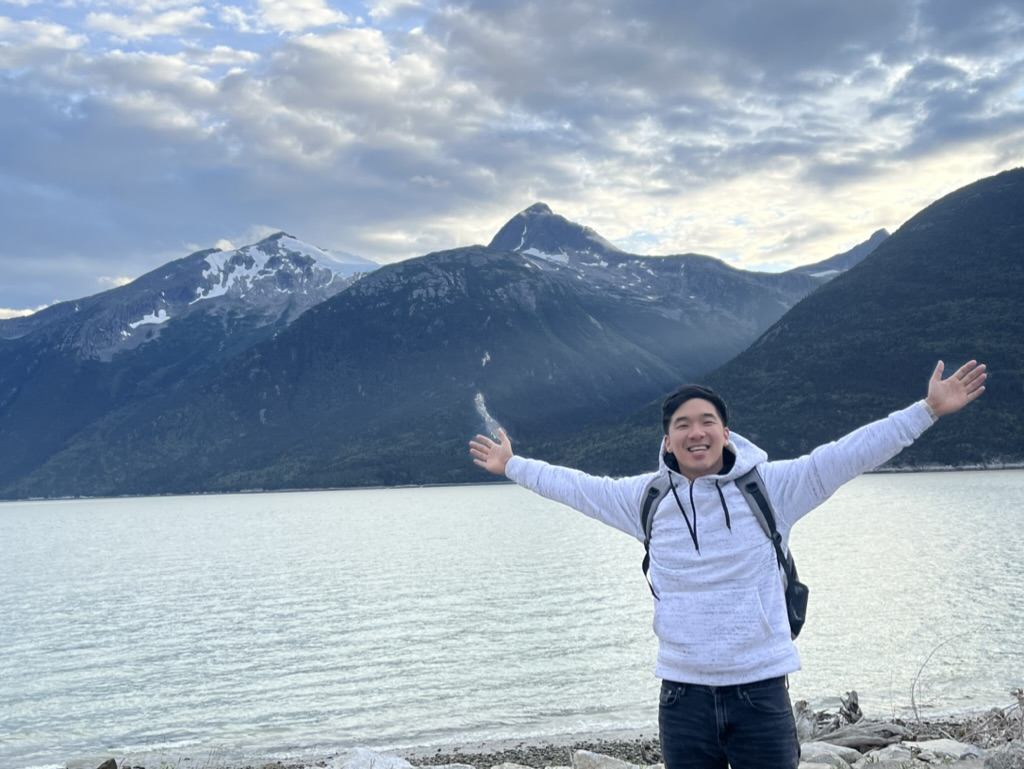
\includegraphics{assets/Picture.jpeg}};
\end{tikzpicture}
}
\hspace{1mm}
\parbox{\dimexpr\linewidth-2.8cm\relax}{
\begin{tabularx}{\linewidth}{L r} \\
    \textbf{\Large \name} \\
    \hline \\ 
    \textbf{Software Engineer | Data Engineer} & {\raisebox{0.0\height}{\footnotesize \faPhone}\ \phone} \\
    {U.S. Citizen} & \href{mailto:\email}{\raisebox{0.0\height}{\footnotesize \faEnvelope}\ {\email}} \\
    \city & {Socials: }{\href{https://leekevinm.com}{\raisebox{0.0\height}{\footnotesize \faGlobe}\ {}} 
        \href{https://github.com/LeeKevinM97}{\raisebox{0.0\height}{\footnotesize \faGithub}\ {}} 
        \href{https://www.linkedin.com/in/leekevinmaximiliano/}{\raisebox{0.0\height}{\footnotesize \faLinkedin}\ {}}}
    \\
\end{tabularx}
}

% %-----------SUMMARY-----------
% \section{\textbf{Summary / Objective}}
% {Motivated Master's in Computer Science candidate adept at data analytics, API development, 
% and system architecture on AWS/Azure. Seeking a role in Software Development or Data Engineering 
% to leverage and expand my skills, driving innovation and efficiency in real-world applications.}

%-----------EXPERIENCE-----------------
\section{\textbf{Experience}}
\resumeSubHeadingListStart

  \resumeExperience
    {CommandLink}{Austin, TX (Remote)}
    {Full-Stack Software Developer}{12/2023 - Present}
    {}
    \vspace{1.0mm}
    \resumeItemListStart
      \resumeProjectSubheader{CommandSecurity}{Ansible, FastAPI, Laravel, React, MySQL, OpenSearch, Celery, Jenkins}
      \item {Migrated legacy PHP Yii services to Python FastAPI microservices for the CommandSecurity platform}
      \item {Normalized EAV-modeled data into relational MySQL schemas, improving backend query performance and maintainability}
      \item {Moved customer sync from request-time triggers to Celery event jobs, reducing API load and sync failures}
      \item {Integrated endpoint detection and response (EDR), cloud infrastructure, and email security tools}
      \item {Centralized security actions, alerts, and asset visibility in CommandSecurity as a single pane of glass}
      \item {Built observability and product analytics workflows with Graylog, Prometheus, Grafana, and PostHog}
      \item {Built Jenkins CI/CD pipelines for Docker builds, ACR publishing, and Azure Container Apps deployments}
      \item {Supported first-year CommandSecurity growth to \$305K annual revenue, 11 customers, and 435 managed assets}
      \resumeProjectSubheader{KnowledgeBase}{Terraform, FastAPI, Swagger, CosmosDB, Blob Storage, Cognitive Search, Docker}
      \item {Provisioned Azure backend infrastructure with Terraform across Cosmos DB, Blob Storage, and Cognitive Search}
      \item {Built FastAPI services for KnowledgeBase content APIs, platform integrations, and Swagger-documented endpoints}
      \item {Implemented hybrid vector and keyword retrieval in Azure Cognitive Search for more relevant article discovery}
    \resumeItemListEnd

  \resumeExperience
    {International Public Safety Data Institute}{Austin, TX (Remote)}
    {Software Developer (Volunteer, Non-Profit; Outside Full-Time Role)}{07/2023 - Present}
    {\textit{npm, TypeScript, AWS (Lambda, S3, CloudWatch), RabbitMQ, Elasticsearch, Grafana, Sentry}}
    \resumeItemListStart
      \item {Modernized fire-service analytics pipelines used for accreditation, reporting, and operational planning}
      \item {Migrated RMS/CAD Lambda functions and normalizers for the NERIS transition from NFIRS}
      \item {Integrated geographic, weather, census, parcel, and SHP data sources for regional incident enrichment}
      \item {Standardized incident data transformations across TypeScript ETL workflows}
      \item {Improved CloudWatch logging and Sentry visibility, accelerating production data debugging}
    \resumeItemListEnd

  \resumeExperience
    {Samsung Austin Semiconductor, LLC.}{Austin, TX (Hybrid)}
    {Engineer II}{06/2018 - 12/2023}
    {\textit{Data Analytics, Python, FastAPI, Streamlit, VBA, Bash Script}}
    \resumeItemListStart
      \item {Co-established the Data Solutions subteam and built chat commands for faster engineering information access}
      \item {Built Big Data process-parameter dashboards that improved workflow monitoring and engineering decisions}
      \item {Automated recurring engineering workflows with FastAPI, VBA, and batch scripts, saving approx. 3 engineer-hours/day}
      \item {Mentored new engineers on system workflows, defect analysis, and production troubleshooting}
      \item {Saved \$400K/year by optimizing residual gas analysis (RGA) process cleans and reducing material waste}
    \resumeItemListEnd

\resumeSubHeadingListEnd

%-----------PROJECTS-----------------
\section{\textbf{Personal Projects}}
\resumeSubHeadingListStart
  \resumeProject
    {\href{https://clearviewatx.com}{ClearView Vision}} % project name (linked)
    {04/2023 - 08/2023} % dates
    {\textit{React, TailwindCSS, Figma, GitHub Pages, GoDaddy}}
    \vspace{0.4mm}
  \resumeItemListStart
    \item {Designed and built a production React website for a local optometry practice}
    \item {Translated Figma wireframes into responsive TailwindCSS components through iterative client feedback}
    \item {Configured domain, DNS, SSL, and GitHub Pages hosting for \href{https://clearviewatx.com}{\textit{clearviewatx.com}}}
  \resumeItemListEnd
\resumeSubHeadingListEnd

%-----------EDUCATION-----------
\section{\textbf{Education}}
\resumeSubHeadingListStart
  \resumeEducation
    {Master of Science in Computer Science}{, Machine Learning Specialization}{GPA: 3.80 / 4.00}
    {Georgia Institute of Technology}{01/2022 - 12/2024}

  \resumeEducation
    {Bachelor of Science in Mechanical Engineering}{, Business Foundations Certificate Program}{GPA: 3.83 / 4.00}
    {The University of Texas at Austin}{08/2015 - 05/2018}
\resumeSubHeadingListEnd

\end{document}
